\chapter{ميكانيك لاغرانج}\label{ch:b3:lagrangian-mechanics}

حاول أن تكتب قانون نيوتن لبندول مزدوج: قوتا شدّ لا تُعرف أيّ منهما
سلفًا، وكلتاهما تغيّر اتجاهها في كل لحظة، وأربع معادلات سلّمية يجب
فكّ اشتباكها لمجرد معرفة كيف تتطور زاويتان. ثم افعل الشيء نفسه من
أجل خرزة على حلقة دوّارة، أو سلسلة من النوابض المتقارنة، أو ذراع
آلية. فالقوى التي تحفظ تماسك الجملة --- من قضبان وسكك ومفاصل ---
لا تؤدي أيّ شغل، ومع ذلك تُلزمنا طريقة نيوتن بحملها في كل حساب.
يعرض هذا الفصل الصياغة التي نشرها لاغرانج سنة 1788: نصف الجملة
بالإحداثيات القليلة التي يمكنها أن تتغير فعلًا، ونكتب دالة واحدة
$L = E_k - E_p$، فتعطي وصفة واحدة معادلات الحركة في أيّ إحداثيات،
وقد حُذف كل قضيب وكل سكة سلفًا. والأفضل من ذلك أن الصياغة الجديدة
تُظهر ما تخفيه صياغة نيوتن: فكل تناظر في $L$ يعطي مقدارًا محفوظًا
--- كمية الحركة من تجانس الفضاء، والطاقة من تجانس الزمن --- وهي
نتيجة لإيمي نويتر غدت المبدأ المنظّم للفيزياء في ميادين تتجاوز
الميكانيك بكثير.

\section{من القوى إلى الإحداثيات}

\begin{definition}[القيود ودرجات الحرية والإحداثيات المعمّمة]\label{def:b3:lagrangian-mechanics:coordinates}
\index{قيد}\index{درجات الحرية}\index{إحداثيات معمّمة}
\emph{القيد} شرط هندسي مفروض على مواضع جملة --- فالخرزة تبقى على
سلكها، وقضيب البندول يحفظ طولًا ثابتًا، وعجلتا محور واحد تدوران
معًا. والقيد الذي يمكن التعبير عنه بمعادلة
$f(\vect r_1, \dots, \vect r_N, t) = 0$ بين الإحداثيات (وربما الزمن
أيضًا) يسمّى \emph{هولونوميًا}. وعدد الطرق المستقلة التي ما زال
التشكيل قادرًا على التغير بها هو عدد \emph{درجات الحرية} $n$؛ وكل
جملة من $n$ مقادير مستقلة $q_1, \dots, q_n$ تحدّد التشكيل تحديدًا
تامًّا هي جملة \emph{إحداثيات معمّمة} --- زوايا أو أطوال أو أيّ خليط
مناسب. ومشتقاتها بالنسبة إلى الزمن $\dot q_1, \dots, \dot q_n$ هي
\emph{السرعات المعمّمة}\index{سرعات معمّمة}.
\end{definition}

\begin{example}[إحصاء درجات الحرية]\label{ex:b3:lagrangian-mechanics:counting}
نقطة على طاولة: $n = 2$. بندول مستوٍ ثابت الطول: زاوية واحدة،
$n = 1$. بندول مزدوج: زاويتان، $n = 1 + 1 = 2$. خرزة على حلقة صلبة:
زاوية واحدة، $n = 1$ --- حتى لو أُجبرت الحلقة نفسها على الدوران،
لأن الدوران المفروض لا يضيف أيّ حرية. جسم صلب حر في الفضاء: ثلاثة
إحداثيات لمركزه وثلاث زوايا، $n = 6$. غاز من $N$ جزيئة حرة (نقاط):
$n = 3N$. وكل \omterm{def:b3:lagrangian-mechanics:coordinates}{قيد} هولونومي يحذف درجة حرية واحدة: فنقطتان يربطهما
قضيب لهما $3 + 3 - 1 = 5$.
\end{example}

\begin{omfigure}
\begin{tikzpicture}[font=\small, >=Stealth]
  % (a) plane pendulum
  \begin{scope}
    \draw[thick] (-1,0) -- (1,0);
    \foreach \i in {-0.8,-0.5,-0.2,0.1,0.4,0.7} \draw (\i,0) -- (\i+0.18,0.16);
    \fill (0,0) circle (1.5pt);
    \draw[dashed] (0,0) -- (0,-2.2);
    \draw[thick] (0,0) -- (-55:2.1);
    \fill[omDef] (-55:2.1) circle (3pt);
    \draw[->] (0,-1.0) arc (-90:-55:1.0);
    \node at (-72:1.35) {$\theta$};
    \node at (-55:2.5) {$m$};
    \node at ($(-55:1.35)+(0.28,0.12)$) {$\ell$};
    \node at (0,-2.9) {إحداثي واحد: $\theta$};
  \end{scope}
  % (b) bead on rotating hoop
  \begin{scope}[xshift=6.2cm]
    \coordinate (C) at (0,-2.35);
    \draw[thick] (C) circle (1.55);
    \draw[dashed] (0,-0.3) -- (0,-4.6);
    \draw[->, thick] (0.35,-0.15) arc (20:160:0.37);
    \node at (0,0.25) {$\omega$};
    \fill (C) circle (1pt);
    \draw (C) -- ++(-50:1.55);
    \fill[omDef] ($(C)+(-50:1.55)$) circle (3pt);
    \draw[->] ($(C)+(0,-0.85)$) arc (-90:-50:0.85);
    \node at ($(C)+(-70:1.18)$) {$\theta$};
    \node at ($(C)+(-38:2.0)$) {$m$};
    \draw (C) -- ++(135:1.55);
    \node at (-1.35,-1.35) {$R$};
    \node at (0,-4.95) {إحداثي واحد: $\theta$};
  \end{scope}
  % (c) double pendulum
  \begin{scope}[xshift=11.4cm]
    \draw[thick] (-0.9,0) -- (0.9,0);
    \foreach \i in {-0.7,-0.4,-0.1,0.2,0.5} \draw (\i,0) -- (\i+0.18,0.16);
    \fill (0,0) circle (1.5pt);
    \draw[dashed] (0,0) -- (0,-1.7);
    \draw[thick] (0,0) -- (-65:1.5) coordinate (m1);
    \fill[omDef] (m1) circle (2.6pt);
    \draw[dashed] (m1) -- ++(0,-1.5);
    \draw[thick] (m1) -- ++(-40:1.5) coordinate (m2);
    \fill[omThm] (m2) circle (2.6pt);
    \draw[->] (0,-0.8) arc (-90:-65:0.8);
    \node at (-80:1.1) {$\theta_1$};
    \draw[->] ($(m1)+(0,-0.75)$) arc (-90:-40:0.75);
    \node at ($(m1)+(-68:1.05)$) {$\theta_2$};
    \node at (0.3,-3.4) {إحداثيان: $\theta_1, \theta_2$};
  \end{scope}
\end{tikzpicture}

{\small \omterm{def:b3:lagrangian-mechanics:coordinates}{الإحداثيات المعمّمة}: تُوصف كل جملة بالزوايا التي يمكنها أن
تتغير فعلًا، لا بالإحداثيات الديكارتية لكتلها. ولا تظهر فيها قط
شدّات القضبان ولا ردّ \omterm{def:b3:lagrangian-mechanics:action}{فعل} الحلقة الناظمي.}
\end{omfigure}

\section{مبدأ الفعل الأصغري}

\begin{definition}[اللاغرانجية والفعل]\label{def:b3:lagrangian-mechanics:action}
\index{لاغرانجية}\index{فعل}
\emph{اللاغرانجية} لجملة ميكانيكية تشتق قواها من طاقة كامنة $E_p$
هي دالة الإحداثيات والسرعات، وربما الزمن أيضًا
\[
L(q, \dot q, t) = E_k - E_p ,
\]
أي الطاقة الحركية \emph{ناقص} الطاقة الكامنة، معبَّرًا عنهما
\omterm{def:b3:lagrangian-mechanics:coordinates}{بالإحداثيات المعمّمة}. و\emph{الفعل} لحركة متصورة $q(t)$ بين طرفين
ثابتين $q(t_1)$ و $q(t_2)$ هو العدد
\[
S[q] = \int_{t_1}^{t_2} L\big(q(t), \dot q(t), t\big)\,\dd t .
\]
والفعل $S$ \emph{دالّية}: تبتلع مسلكًا كاملًا وتعيد عددًا واحدًا،
بواحدة الجول-ثانية --- وهي واحدة ثابت بلانك.
\end{definition}

\begin{theorem}[مبدأ هاميلتون ومعادلات أويلر--لاغرانج]\label{thm:b3:lagrangian-mechanics:euler-lagrange}
\index{مبدأ هاميلتون}\index{معادلات أويلر--لاغرانج}\index{الفعل الأصغري}
من بين جميع الحركات المتصورة التي تصل الطرفين نفسيهما في الزمن
نفسه، الحركة الفعلية هي التي تجعل \omterm{def:b3:lagrangian-mechanics:action}{الفعل} \emph{مستقرًا}
(\emph{\omterm{thm:b3:lagrangian-mechanics:euler-lagrange}{مبدأ هاميلتون}}، أو مبدأ \emph{\omterm{thm:b3:lagrangian-mechanics:euler-lagrange}{الفعل الأصغري}}). وعلى نحو
مكافئ، تحقق الحركة \emph{\omterm{thm:b3:lagrangian-mechanics:euler-lagrange}{معادلات أويلر--لاغرانج}}
\[
\frac{\dd}{\dd t}\frac{\partial L}{\partial\dot q_i}
 - \frac{\partial L}{\partial q_i} = 0 ,
\qquad i = 1, \dots, n :
\]
أي معادلة واحدة من المرتبة الثانية لكل درجة حرية، في أيّ إحداثيات
اختيرت.
\end{theorem}

\begin{proof}
نشوّه المسلك: $q_i(t) \to q_i(t) + \delta q_i(t)$ مع
$\delta q_i(t_1) = \delta q_i(t_2) = 0$. وحتى المرتبة الأولى،
\[
\delta S = \int_{t_1}^{t_2}\sum_i\Big(
  \frac{\partial L}{\partial q_i}\,\delta q_i
 + \frac{\partial L}{\partial\dot q_i}\,\delta\dot q_i\Big)\dd t
 = \int_{t_1}^{t_2}\sum_i\Big(
  \frac{\partial L}{\partial q_i}
 - \frac{\dd}{\dd t}\frac{\partial L}{\partial\dot q_i}\Big)\delta q_i\,\dd t ,
\]
بعد مكاملة الحد الثاني بالتجزئة ($\delta\dot q_i =
\dd(\delta q_i)/\dd t$) وإهمال الحد الحدّي الذي ينعدم عند الطرفين
الثابتين. فإذا كان $\delta S = 0$ من أجل \emph{كل} تشويه، وجب أن
ينعدم القوس في كل لحظة ومن أجل كل $i$ --- إذ لو كان موجبًا في
موضع ما لأعطى نتوء $\delta q_i$ مركَّز هناك $\delta S \neq 0$.
والعكس يُقرأ من السطر نفسه.
\end{proof}

\begin{omfigure}
\begin{tikzpicture}[font=\small, >=Stealth]
  \draw[->] (0,0) -- (7.6,0) node[right] {$t$};
  \draw[->] (0,0) -- (0,3.4) node[above] {$q$};
  \fill (0.8,0.7) circle (2pt) node[below left] {$q(t_1)$};
  \fill (6.8,2.3) circle (2pt) node[above right] {$q(t_2)$};
  \draw[omDef, very thick] (0.8,0.7) .. controls (2.6,2.6) and (5.0,1.4) .. (6.8,2.3);
  \draw[omExo, dashed] (0.8,0.7) .. controls (2.2,0.6) and (5.4,0.9) .. (6.8,2.3);
  \draw[omExo, dashed] (0.8,0.7) .. controls (3.0,3.6) and (5.2,2.9) .. (6.8,2.3);
  \node[omDef] at (1.9,3.35) {المسلك الفعلي};
  \draw[->, omDef] (2.25,3.15) -- (2.85,2.3);
  \node[omExo] at (3.4,0.42) {مسالك متغيَّرة};
  \draw[<->] (4.1,1.62) -- (4.1,2.62);
  \node at (4.55,2.15) {$\delta q$};
\end{tikzpicture}

{\small \omterm{thm:b3:lagrangian-mechanics:euler-lagrange}{مبدأ هاميلتون}: من بين كل المسالك ذات الطرفين نفسيهما
والمدة نفسها، الفعلي منها هو الذي يجعل $S = \int L\,\dd t$ مستقرًا
--- فالتشويهات من المرتبة الأولى $\delta q$ لا تغيّر $S$ إلا في
المرتبة الثانية.}
\end{omfigure}

\begin{proposition}[استعادة نيوتن]\label{prop:b3:lagrangian-mechanics:newton}
من أجل جسيم بالإحداثيات الديكارتية، $L = \tfrac12 m(\dot x^2 +
\dot y^2 + \dot z^2) - E_p(x,y,z)$، وتُكتب \omterm{thm:b3:lagrangian-mechanics:euler-lagrange}{معادلات أويلر--لاغرانج}
$m\ddot x = -\partial E_p/\partial x$ وكذلك من أجل $y$ و $z$: أي
$m\vect a = \vect F$ بالضبط. فميكانيك لاغرانج وميكانيك نيوتن
متوافقان حيثما صحّ كلاهما؛ غير أن الصياغة الجديدة تصمد لتغيير
الإحداثيات، وهو ما لا تصمد له معادلات نيوتن بمركباتها.
\end{proposition}

\begin{proof}
لدينا $\partial L/\partial\dot x = m\dot x$ و $\partial L/\partial x =
-\partial E_p/\partial x$؛ ومعادلة أويلر--لاغرانج هي
$\dd(m\dot x)/\dd t + \partial E_p/\partial x = 0$.
\end{proof}

\begin{remark}[لماذا تختفي قوى القيد]\label{rem:b3:lagrangian-mechanics:constraints}
شدّة القضيب، وردّ \omterm{def:b3:lagrangian-mechanics:action}{فعل} السكة الناظمي، تعملان عموديًا على كل انتقال
يسمح به \omterm{def:b3:lagrangian-mechanics:coordinates}{القيد}: فلا تؤديان أيّ شغل في حركة توافق \omterm{def:b3:lagrangian-mechanics:coordinates}{القيد}. ولمّا كان
\omterm{def:b3:lagrangian-mechanics:action}{الفعل} مبنيًا من طاقات لا تُحسب إلا على مثل هذه الحركات، فإن هذه
القوى لا تدخل قط في $L$ --- وتلك هي المعجزة العملية للطريقة.
والتبرير العام (مبدأ دالامبير في الأشغال الافتراضية) مُسلَّم به
هنا؛ وفي كل جملة من جمل هذا الكتاب يمكن التحقق من الوصفة الآتية
أمام نيوتن مباشرة، كما بدأت تفعل
\cref{prop:b3:lagrangian-mechanics:newton}. وإذا أُريدت قوة \omterm{def:b3:lagrangian-mechanics:coordinates}{القيد}
نفسها --- هل ينكسر القضيب؟ --- عدنا إلى نيوتن من أجل تلك القوة
وحدها، والحركة معلومة سلفًا.
\end{remark}

\begin{method}[وصفة لاغرانج]\label{met:b3:lagrangian-mechanics:recipe}
(1) نحصي \omterm{def:b3:lagrangian-mechanics:coordinates}{درجات الحرية} ونختار الإحداثيات $q_i$ --- زوايا من أجل
الدورانات، وفواصل على السكك. (2) نعبّر عن المواضع
$\vect r(q_i, t)$، ونشتقّها لنحصل على السرعات، ونكتب $E_k$؛ ونكتب
$E_p$. (3) $L = E_k - E_p$، مع إهمال أيّ ثابت جمعي. (4) معادلة
أويلر--لاغرانج واحدة لكل إحداثي. (5) قبل الحل، نجني المقادير
المحفوظة: الإحداثيات الدورية
(\cref{def:b3:lagrangian-mechanics:momentum}) \omterm{prop:b3:lagrangian-mechanics:energy}{ودالة الطاقة}
(\cref{prop:b3:lagrangian-mechanics:energy}). (6) نتحقق من الحالات
الحدية: الزوايا الصغيرة، وإيقاف الدوران، والحالات الخاصة المعروفة.
\end{method}

\begin{example}[البندول في ثلاثة أسطر]\label{ex:b3:lagrangian-mechanics:pendulum}
إحداثي واحد $\theta$؛ ولدينا $\vect v = \ell\dot\theta\,\vect e_\theta$،
ومنه $E_k = \tfrac12 m\ell^2\dot\theta^2$ و $E_p = -mg\ell\cos\theta$.
عندئذٍ $L = \tfrac12 m\ell^2\dot\theta^2 + mg\ell\cos\theta$، ومنه
$\dd(m\ell^2\dot\theta)/\dd t = -mg\ell\sin\theta$:
\[
\ddot\theta = -\frac{g}{\ell}\sin\theta ,
\]
وهي المعادلة التي حصل عليها كتاب السنة الأولى من عزم الثقل ---
من دون ذكر الشدّة قط.
\end{example}

\begin{example}[خرزة على حلقة دوّارة]\label{ex:b3:lagrangian-mechanics:hoop}
خرزة كتلتها $m$ تنزلق على حلقة دائرية شاقولية نصف قطرها $R$
مُجبرة على الدوران حول قطرها الشاقولي بسرعة زاوية ثابتة $\omega$
(\cref{ex:b3:lagrangian-mechanics:counting}). لها إحداثي واحد هو
الزاوية القطبية $\theta$ ابتداءً من الأسفل. ولسرعة الخرزة مركبة
$R\dot\theta$ على طول الحلقة ومركبة $\omega R\sin\theta$ ناتجة عن
الدوران المفروض، عمودية عليها:
\[
L = \tfrac12 mR^2\dot\theta^2 + \tfrac12 m\omega^2R^2\sin^2\theta
 + mgR\cos\theta ,
\qquad
mR^2\ddot\theta = m\omega^2R^2\sin\theta\cos\theta - mgR\sin\theta .
\]
مواضع التوازن حيث $\ddot\theta = 0$: الأسفل $\theta = 0$ (والأعلى،
وهو غير مستقر دائمًا)، ثم، عندما يكون $\omega^2 > g/R$، زوج جديد
$\cos\theta_{\text{توازن}} = g/\omega^2R$. وبكتابة المعادلة في الشكل
$mR^2\ddot\theta = -\dd U_{\text{فعّال}}/\dd\theta$ مع
\emph{الطاقة الكامنة الفعّالة}\index{طاقة كامنة فعّالة}
\[
U_{\text{فعّال}}(\theta) = -mgR\cos\theta
 - \tfrac12 m\omega^2R^2\sin^2\theta
\]
تصير الهندسة ظاهرة: فدون السرعة الحرجة
$\omega_{\text{c}} = \sqrt{g/R}$ يكون الأسفل بئرًا؛ وفوقها يصير
الأسفل قمة وتستقر الخرزة على المنحدر، فترتفع كلما دارت الحلقة
أسرع --- وهو مبدأ المنظّم الطاردي الذي كان يضبط الآلات البخارية.
\end{example}

\begin{omfigure}
\begin{tikzpicture}
  \begin{axis}[omaxis, axis x line=bottom, axis y line=left,
    width=11.4cm, height=5.6cm, xmin=-180, xmax=180,
    ymin=-1.65, ymax=1.2, xlabel={$\theta$ (بالدرجات)},
    xlabel style={at={(axis description cs:0.5,-0.1)}, anchor=north},
    ylabel={$U_{\text{فعّال}}/mgR$}, xtick={-180,-90,0,90,180}, ytick=\empty,
    clip=false,
    legend style={font=\scriptsize, at={(0.5,-0.32)}, anchor=north,
      draw=none, fill=none, legend columns=2}]
    \addplot[omDef, thick, domain=-180:180, samples=90]
      {-cos(x) - 0.25*sin(x)^2};
    \addlegendentry{$\omega^2 = g/2R$ (بطيء): بئر عند $\theta = 0$}
    \addplot[omThm, thick, domain=-180:180, samples=90]
      {-cos(x) - 1.0*sin(x)^2};
    \addlegendentry{$\omega^2 = 2g/R$ (سريع): بئران عند $\pm 60^\circ$}
    \fill[omThm] (axis cs:60,-1.25) circle (1.8pt);
    \fill[omThm] (axis cs:-60,-1.25) circle (1.8pt);
    \fill[omDef] (axis cs:0,-1) circle (1.8pt);
  \end{axis}
\end{tikzpicture}

{\small الكمون الفعّال للخرزة على الحلقة الدوّارة. فعندما يتجاوز
$\omega$ القيمة $\sqrt{g/R}$ تنشطر البئر الوحيدة في الأسفل إلى
بئرين متناظرتين: وترتفع زاوية التوازن مع تزايد سرعة الدوران.}
\end{omfigure}

\section{التناظرات وقوانين الانحفاظ}

\begin{definition}[كمية الحركة المعمّمة والإحداثي الدوري]\label{def:b3:lagrangian-mechanics:momentum}
\index{كمية حركة معمّمة}\index{إحداثي دوري}
\emph{كمية الحركة المعمّمة} المرافقة للإحداثي $q_i$ هي
\[
p_i = \frac{\partial L}{\partial\dot q_i} .
\]
من أجل إحداثي ديكارتي هي كمية الحركة العادية $m\dot x$؛ ومن أجل
زاوية هي عزم حركي. والإحداثي الذي لا يظهر في $L$ (وإن ظهرت سرعته)
يسمّى \emph{دوريًا}.
\end{definition}

\begin{proposition}[الإحداثيات الدورية تعطي قوانين انحفاظ]\label{prop:b3:lagrangian-mechanics:cyclic}
إذا كان $q_i$ دوريًا انحفظت كمية حركته المرافقة: فمن
$\partial L/\partial q_i = 0$ ينتج $\dd p_i/\dd t = 0$. واختيار
الإحداثيات بحيث يكون أكبر عدد ممكن منها دوريًا هو أنجع خطوة
منفردة في حل مسألة ميكانيكية.
\end{proposition}

\begin{proof}
مباشرةً من معادلة أويلر--لاغرانج من أجل $q_i$.
\end{proof}

\begin{example}[قوة مركزية تُحل بالنظر]\label{ex:b3:lagrangian-mechanics:central}
جسيم في كمون مركزي $E_p(r)$، بالإحداثيات القطبية في مستوي
حركته:
\[
L = \tfrac12 m(\dot r^2 + r^2\dot\varphi^2) - E_p(r) .
\]
الإحداثي $\varphi$ دوري، ومن ثمّ ينحفظ $p_\varphi = mr^2\dot\varphi$
--- وهو العزم الحركي: أي قانون كبلر في المساحات، الذي اشتقّه كتاب
السنة الأولى من معادلة العزوم، يسقط هنا قبل حل أيّ معادلة.
والمعادلة القطرية المتبقية هي
$m\ddot r = mr\dot\varphi^2 - E_p'(r)$، أي الحركة الأحادية البعد في
الكمون الفعّال $E_p(r) + p_\varphi^2/2mr^2$ الوارد في ذلك
الكتاب.
\end{example}

\begin{theorem}[مبرهنة نويتر]\label{thm:b3:lagrangian-mechanics:noether}
\index{مبرهنة نويتر}\index{تناظر}
لكل تناظر متصل \omterm{def:b3:lagrangian-mechanics:action}{للاغرانجية} مقدار محفوظ يقابله. وبدقة: إذا كان
الانزياح $q_i \to q_i + \varepsilon\,K_i(q)$ يترك $L$ بلا تغيير
حتى المرتبة الأولى في $\varepsilon$ من أجل كل الحركات، فإن
\[
Q = \sum_i p_i\,K_i(q)
\]
ثابت على طول كل حركة فعلية. فتجانس الفضاء (الثبات بالانسحاب) يعطي
كمية الحركة؛ وتماثل مناحي الفضاء (الثبات بالدوران) يعطي العزم
الحركي؛ وتجانس الزمن يعطي الطاقة
(\cref{prop:b3:lagrangian-mechanics:energy}).
\end{theorem}

\begin{proof}
الثبات حتى المرتبة الأولى يعني
$0 = \delta L = \sum_i\big(\partial_{q_i}L\,K_i +
\partial_{\dot q_i}L\,\dot K_i\big)\varepsilon$. وعلى حركة فعلية
لدينا $\partial_{q_i}L = \dot p_i$ بحسب أويلر--لاغرانج، فيكون
القوس $\sum_i(\dot p_iK_i + p_i\dot K_i) = \dd Q/\dd t$. \omterm{def:b3:lagrangian-mechanics:momentum}{والإحداثي
الدوري} هو الحالة الخاصة $K_i = \delta_{ij}$. أما حالة انزياح الزمن
فتحتاج إلى الحساب المستقل الوارد في
\cref{prop:b3:lagrangian-mechanics:energy}؛ والمبرهنة الكاملة، من
أجل تحويلات تغيّر $t$ أيضًا أو تعدّل $L$ بمشتق تام، تُبرهن في
دروس الميكانيك التحليلي وهي مُسلَّم بها هنا في هذا التعميم.
\end{proof}

\begin{proposition}[دالة الطاقة]\label{prop:b3:lagrangian-mechanics:energy}
\index{دالة الطاقة}
على طول أيّ حركة، فإن \emph{\omterm{prop:b3:lagrangian-mechanics:energy}{دالة الطاقة}}
\[
h = \sum_i \dot q_i\,\frac{\partial L}{\partial\dot q_i} - L
\qquad\text{تحقق}\qquad
\frac{\dd h}{\dd t} = -\frac{\partial L}{\partial t} .
\]
فإذا لم تتعلق $L$ بالزمن صراحةً انحفظت $h$. وإذا كانت العلاقات
$\vect r(q)$ بين المواضع والإحداثيات خالية من الزمن أيضًا --- لا
دوران مفروض ولا سند متحرك --- كانت $E_k$ شكلًّا تربيعيًا في
$\dot q_i$ وكان $h = E_k + E_p$: أي الطاقة الميكانيكية. أما مع \omterm{def:b3:lagrangian-mechanics:coordinates}{قيد}
متعلق بالزمن فتبقى $h$ محفوظة عندما يكون
$\partial L/\partial t = 0$، لكنها \emph{ليست} الطاقة: إذ يتبادل
المحرك الذي يفرض \omterm{def:b3:lagrangian-mechanics:coordinates}{القيد} الشغل مع الجملة.
\end{proposition}

\begin{proof}
$\dd h/\dd t = \sum_i(\ddot q_ip_i + \dot q_i\dot p_i) -
\sum_i(\partial_{q_i}L\,\dot q_i + \partial_{\dot q_i}L\,\ddot q_i) -
\partial_tL$. تتلاشى الحدود في $\ddot q_i$؛ وتحوّل \omterm{thm:b3:lagrangian-mechanics:euler-lagrange}{معادلات
أويلر--لاغرانج} $\dot p_i$ إلى $\partial_{q_i}L$ فيتلاشى الزوج
التالي؛ ويبقى $-\partial_tL$. وإذا كان $E_k = \tfrac12\sum a_{jk}(q)\dot
q_j\dot q_k$ أعطت متطابقة أويلر للأشكال التربيعية $\sum\dot
q_i\,\partial E_k/\partial\dot q_i = 2E_k$، ومنه $h = 2E_k - (E_k - E_p)
= E_k + E_p$.
\end{proof}

\begin{example}[الحلقة الدوّارة تحفظ $h$ لا $E$]\label{ex:b3:lagrangian-mechanics:hoop-energy}
من أجل خرزة \cref{ex:b3:lagrangian-mechanics:hoop}، ليس في $L$
زمن $t$ صريح، ومن ثمّ ينحفظ $h = \tfrac12 mR^2\dot\theta^2 + U_{\text{فعّال}}
(\theta)$ --- لكن الطاقة الميكانيكية $E = \tfrac12
mR^2\dot\theta^2 + \tfrac12 m\omega^2R^2\sin^2\theta - mgR\cos\theta$
لا تنحفظ: إذ يتغير $E = h + m\omega^2R^2\sin^2\theta$ كلما انزلقت
الخرزة. والفرق هو شغل المحرك الذي يبقي $\omega$ ثابتة بينما تتغير
مسافة الخرزة عن المحور.
\end{example}

\section{الجسيمات المشحونة والاهتزازات الصغيرة}

\begin{proposition}[لاغرانجية جسيم مشحون]\label{prop:b3:lagrangian-mechanics:charge}
\index{كمون متعلق بالسرعة}
في مجال كهرطيسي موصوف بالكمونين $V$ و
$\vect A$ (مع $\vect E = -\vect\nabla V - \partial_t\vect A$ و
$\vect B = \operatorname{\vect{curl}}\vect A$، كما في كتاب السنة
الثانية)، تعطي \omterm{def:b3:lagrangian-mechanics:action}{اللاغرانجية}
\[
L = \tfrac12 m\vect v^{\,2} - qV + q\,\vect v\cdot\vect A
\]
بواسطة \omterm{thm:b3:lagrangian-mechanics:euler-lagrange}{معادلات أويلر--لاغرانج} قوة لورنتز بالضبط
$m\dot{\vect v} = q(\vect E + \vect v\wedge\vect B)$. فالقوة
المغناطيسية، التي لا تؤدي شغلًا ولا تشتق من طاقة كامنة عادية،
تدخل عبر حدّ خطي في السرعة؛ وتصير كمية الحركة المرافقة
$\vect p = m\vect v + q\vect A$، ولم تعد
$m\vect v$ وحدها.
\end{proposition}

\begin{proof}
من أجل المركبة $x$: $p_x = m\dot x + qA_x$، و
$\partial_xL = -q\,\partial_xV + q\,\vect v\cdot\partial_x\vect A$.
وتعطي معادلة أويلر--لاغرانج $m\ddot x = -q\,\partial_xV -
q\,\dd A_x/\dd t + q\,\vect v\cdot\partial_x\vect A$. وعلى الحركة
$\dd A_x/\dd t = \partial_tA_x + (\vect v\cdot\vect\nabla)A_x$، ومنه
$m\ddot x = qE_x + q\big[\vect v\cdot\partial_x\vect A - (\vect v\cdot
\vect\nabla)A_x\big]$، والقوس هو المركبة $x$ للمقدار $\vect
v\wedge(\vect\nabla\wedge\vect A) = \vect v\wedge\vect B$ --- انشر
كليهما للتحقق.
\end{proof}

\begin{proposition}[الاهتزازات الصغيرة والأنماط الذاتية]\label{prop:b3:lagrangian-mechanics:modes}
\index{أنماط ذاتية}\index{اهتزازات صغيرة}
بجوار توازن مستقر $q^{\text{توازن}}$، ننشر $L$ حتى المرتبة الثانية
في الانزياحات $u_i = q_i - q_i^{\text{توازن}}$:
$L \approx \tfrac12\sum m_{ij}\dot u_i\dot u_j -
\tfrac12\sum k_{ij}u_iu_j$ بمصفوفتين متناظرتين ثابتتين. فتكون
معادلات الحركة خطية، وتكون كل حركة تراكبًا من
\emph{\omterm{prop:b3:lagrangian-mechanics:modes}{الأنماط الذاتية}}: اهتزازات جماعية $u_i(t) = a_i\cos(\Omega t
+ \phi)$ تهتز فيها الإحداثيات كلها بتواتر واحد مشترك، وتحقق
السعات والتواترات $\sum_j(k_{ij} -
\Omega^2m_{ij})\,a_j = 0$ --- وهي مسألة قيم ذاتية لمصفوفة، ولها $n$
نمطًا من أجل $n$ درجة حرية.
\end{proposition}

\begin{proof}
تنعدم الحدود الخطية عند التوازن؛ وتُكتب \omterm{thm:b3:lagrangian-mechanics:euler-lagrange}{معادلات أويلر--لاغرانج}
للدالة $L$ التربيعية $\sum_jm_{ij}\ddot u_j = -\sum_jk_{ij}u_j$.
وإدخال الاهتزاز التجريبي يعطي الجملة الخطية المذكورة، التي ليس
لها متجهة سعات غير معدومة إلا عندما يكون $\det(k_{ij} -
\Omega^2m_{ij}) = 0$: أي $n$ قيمة للمقدار $\Omega^2$، جميعها موجبة
عند توازن مستقر. وأما كون الحركة العامة تراكبًا من الأنماط فهو
قطر جملة من شكلين تربيعيين، وهي نتيجة من الجبر الخطي في كتاب
الرياضيات للسنة الثانية؛ والتمام مُسلَّم به.
\end{proof}

\begin{example}[بندولان متقارنان بنابض]\label{ex:b3:lagrangian-mechanics:coupled}
بندولان متماثلان (الكتلة $m$، الطول $\ell$)، كرتاهما موصولتان
بنابض صلابته $k$ يكون مرتخيًا حين يتدليان شاقوليًا. ومن أجل
الزوايا الصغيرة،
\[
L = \tfrac12 m\ell^2(\dot\theta_1^2 + \dot\theta_2^2)
 - \tfrac12 mg\ell(\theta_1^2 + \theta_2^2)
 - \tfrac12 k\ell^2(\theta_2 - \theta_1)^2 .
\]
يوحي التناظر بالتركيبين $s = \theta_1 + \theta_2$ و $d =
\theta_1 - \theta_2$ اللذين يفصلان المعادلتين: \emph{النمط المتوافق
في الطور} ($\theta_1 = \theta_2$، والنابض خامل) عند $\Omega_1 =
\sqrt{g/\ell}$، و\emph{النمط المتعاكس} ($\theta_1 = -\theta_2$،
والنابض ممدود مرتين) عند $\Omega_2 = \sqrt{g/\ell + 2k/m}$. وأطلق
بندولًا واحدًا --- وهو خليط متساوٍ من النمطين --- فتهاجر الطاقة
كلها من بندول إلى الآخر ثم تعود بتواتر النبضات
$(\Omega_2 - \Omega_1)/2\pi$: وهي تجربة البندولين المتقارنين،
والآلية الكامنة وراء كل انتقال للطاقة بالرنين، من الدارات
المُوالَفة إلى الاهتزازات الجزيئية.
\end{example}

\begin{omfigure}
\begin{tikzpicture}[font=\small, >=Stealth]
  % in-phase mode
  \begin{scope}
    \draw[thick] (-0.4,0) -- (3.4,0);
    \foreach \i in {-0.2,0.3,0.8,1.3,1.8,2.3,2.8} \draw (\i,0) -- (\i+0.18,0.16);
    \fill (0.5,0) circle (1.2pt);
    \fill (2.5,0) circle (1.2pt);
    \draw[thick] (0.5,0) -- ++(-75:1.9) coordinate (a1);
    \draw[thick] (2.5,0) -- ++(-75:1.9) coordinate (a2);
    \fill[omDef] (a1) circle (2.6pt);
    \fill[omDef] (a2) circle (2.6pt);
    \draw[decorate, decoration={coil, aspect=0.6, segment length=3pt, amplitude=2pt}] (a1) -- (a2);
    \draw[->, omDef] ($(a1)+(0.05,-0.3)$) -- ++(0.5,0);
    \draw[->, omDef] ($(a2)+(0.05,-0.3)$) -- ++(0.5,0);
    \node at (1.5,-2.9) {متوافقان في الطور: $\Omega_1 = \sqrt{g/\ell}$};
  \end{scope}
  % opposed mode
  \begin{scope}[xshift=6.4cm]
    \draw[thick] (-0.4,0) -- (3.4,0);
    \foreach \i in {-0.2,0.3,0.8,1.3,1.8,2.3,2.8} \draw (\i,0) -- (\i+0.18,0.16);
    \fill (0.5,0) circle (1.2pt);
    \fill (2.5,0) circle (1.2pt);
    \draw[thick] (0.5,0) -- ++(-105:1.9) coordinate (b1);
    \draw[thick] (2.5,0) -- ++(-75:1.9) coordinate (b2);
    \fill[omThm] (b1) circle (2.6pt);
    \fill[omThm] (b2) circle (2.6pt);
    \draw[decorate, decoration={coil, aspect=0.6, segment length=5pt, amplitude=2pt}] (b1) -- (b2);
    \draw[->, omThm] ($(b1)+(-0.05,-0.3)$) -- ++(-0.5,0);
    \draw[->, omThm] ($(b2)+(0.05,-0.3)$) -- ++(0.5,0);
    \node at (1.5,-2.9) {متعاكسان: $\Omega_2 = \sqrt{g/\ell + 2k/m}$};
  \end{scope}
\end{tikzpicture}

{\small النمطان الذاتيان للبندولين المتقارنين. ففي حالة التوافق
في الطور لا يمتد النابض أبدًا ويكون التواتر تواتر البندول الحر؛
وفي حالة التعاكس تشعر كل كرة بالنابض مضاعفًا.}
\end{omfigure}

\begin{omfigure}
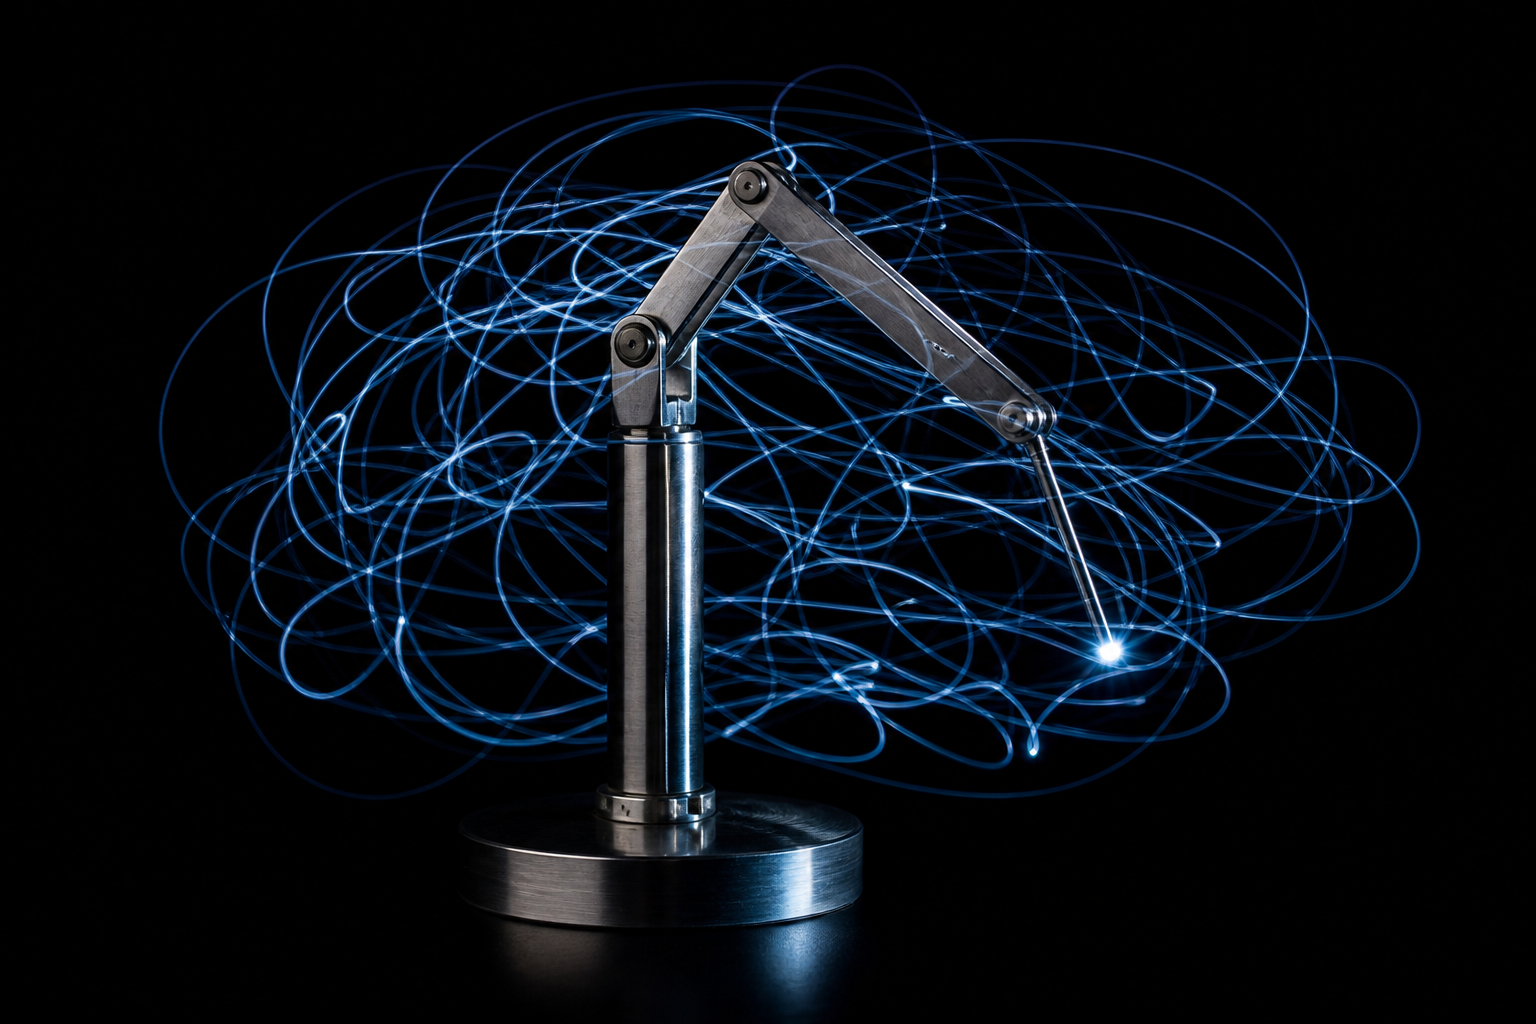
\includegraphics[width=0.58\linewidth]{images/book5/ai/b5-01-double-pendulum-trace.png}

{\small بندول مزدوج مرسوم بتعريض ضوئي طويل: إحداثيان، \omterm{def:b3:lagrangian-mechanics:action}{ولاغرانجية} واحدة، وحركة لا تتنبأ بها أيّ صيغة زمنًا طويلًا --- فآلة \omterm{thm:b3:lagrangian-mechanics:euler-lagrange}{الفعل الأصغري} في هذا الفصل تكتب المعادلات، والفوضى تُبقي حلولها متواضعة.}
\end{omfigure}

\section{تمارين}

\begin{exercise}[$\star$]\label{exo:b3:lagrangian-mechanics:1}
أحصِ \omterm{def:b3:lagrangian-mechanics:coordinates}{درجات الحرية} واقترح \omterm{def:b3:lagrangian-mechanics:coordinates}{إحداثيات معمّمة}: (أ) جسيم داخل وعاء
ثابت؛ (ب) أسطوانة تتدحرج من دون انزلاق على مستوٍ مائل ثابت؛ (ج)
بندول مزدوج ينزلق محوره العلوي على سكة أفقية؛ (د) ثقالة (كتلتان
وقضيب صلب) في الفضاء؛ (ه) خرزتان على السلك الدائري الثابت نفسه.
أيّ \omterm{def:b3:lagrangian-mechanics:coordinates}{قيد} في هذه القائمة يربط بين السرعات لا بين المواضع، ولماذا
يمكن مع ذلك مكاملته ليصير هولونوميًا؟
\end{exercise}

\begin{exercise}[$\star$]\label{exo:b3:lagrangian-mechanics:2}
من أجل البندول المستوي (\cref{ex:b3:lagrangian-mechanics:pendulum}):
(أ) تحقق من أبعاد $L$ ومن أبعاد $p_\theta =
\partial L/\partial\dot\theta$؛ (ب) عيّن $p_\theta$ فيزيائيًّا؛ (ج)
استنتج دور \omterm{prop:b3:lagrangian-mechanics:modes}{الاهتزازات الصغيرة}؛ (د) احسب \omterm{def:b3:lagrangian-mechanics:action}{الفعل} $S$ لاهتزازة صغيرة
كاملة سعتها $\theta_0$ --- وفسّر النتيجة قبل الحساب (ما المتوسط
الزمني للمقدار $E_k - E_p$ في اهتزاز توافقي؟).
\end{exercise}

\begin{exercise}[$\star$]\label{exo:b3:lagrangian-mechanics:3}
آلة أتوود: كتلتان $m_1$ و $m_2$ معلقتان بخيط مثالي على بكرة عديمة
الكتلة. (أ) اختر إحداثيًا واحدًا واكتب $L$. (ب) أوجد التسارع. (ج)
احتاجت معالجة نيوتن إلى الشدّة --- فأين ذهبت؟ (د) كيف تستعيد
الشدّة متى عُرفت الحركة؟
\end{exercise}

\begin{exercise}[$\star$]\label{exo:b3:lagrangian-mechanics:4}
جسيم حر بالإحداثيات الأسطوانية: $L = \tfrac12 m(\dot r^2 +
r^2\dot\varphi^2 + \dot z^2)$. (أ) ما الإحداثيات الدورية، وما
كميات الحركة المحفوظة؟ (ب) لماذا \emph{لا} ينحفظ $p_r$ مع أن لا
قوة تؤثر؟ (ج) اكتب معادلة أويلر--لاغرانج من أجل $r$ وفسّر الحدّ
$mr\dot\varphi^2$. (د) تحقق من أن مستقيمًا يُقطع بسرعة ثابتة
يحققها.
\end{exercise}

\begin{exercise}[$\star\star$]\label{exo:b3:lagrangian-mechanics:5}
كتلة $m$ تنزلق على وجه عديم الاحتكاك (زاويته $\alpha$) لإسفين
كتلته $M$، وهو نفسه حر في الانزلاق على أرض عديمة الاحتكاك. (أ)
اختر إحداثيين: فاصلة الإسفين $X$ ومسافة الكتلة $s$ نزولًا على
الوجه؛ واكتب $L$. (ب) أيّ الإحداثيين دوري، وأيّ قانون انحفاظ
يعبّر عنه؟ (ج) أوجد التسارعين. (د) تحقق من الحالتين الحديتين
$M \to \infty$ و $\alpha \to
90^\circ$.
\end{exercise}

\begin{exercise}[$\star\star$]\label{exo:b3:lagrangian-mechanics:6}
البندول الكروي: كرة على قضيب طوله $\ell$، حرة في الزاويتين
($\theta$ ابتداءً من الشاقول النازل، و $\varphi$ حوله). (أ) اكتب
$L$. (ب) عيّن \omterm{def:b3:lagrangian-mechanics:momentum}{الإحداثي الدوري} والمقدار المحفوظ $p_\varphi$. (ج)
أرجع حركة $\theta$ إلى كمون فعّال وارسمه تقريبيًا. (د) من أجل
الحركة المخروطية $\theta =
\theta_0$، استعد علاقة البندول المخروطي $\cos\theta_0 =
g/\ell\omega^2$ الواردة في كتاب السنة الأولى.
\end{exercise}

\begin{exercise}[$\star\star$]\label{exo:b3:lagrangian-mechanics:7}
بندول (كتلته $m$، طوله $\ell$) معلق بعربة كتلتها $M$ حرة في
التدحرج على سكة أفقية. (أ) بالإحداثيين $X$ (العربة) و $\theta$،
اكتب $L$. (ب) ما المقدار المحفوظ، ولماذا فيزيائيًّا؟ (ج) خطّط من
أجل $\theta$ الصغيرة وبيّن أن تواتر الاهتزاز هو
$\Omega = \sqrt{(1 + m/M)\,g/\ell}$. (د) فسّر الحالتين $M \to
\infty$ و $M \to 0$ --- لماذا \emph{ترفع} العربة الخفيفة التواتر؟
\end{exercise}

\begin{exercise}[$\star\star$]\label{exo:b3:lagrangian-mechanics:8}
جسيم شحنته $q$ في مجال منتظم $\vect B = B\vect e_z$، موصوف
بالكمون $\vect A = \tfrac12\vect B\wedge\vect r$. (أ) اكتب $L$
بالإحداثيات الديكارتية. (ب) استنتج معادلات الحركة وتحقق من أنها
تصف دائرة السيكلوترون عند $\omega_{\text{c}} = qB/m$. (ج) احسب
كميتي الحركة المرافقتين $p_x$ و $p_y$: هل هما $m\dot x$ و
$m\dot y$؟ وهل تنحفظان؟ (د) بيّن أن $L$ مكتوبة بالإحداثيات
الأسطوانية يكون فيها $\varphi$ دوريًا، وعيّن المقدار المحفوظ
$p_\varphi$ من أجل دائرة مركزها على المحور.
\end{exercise}

\begin{exercise}[$\star\star$]\label{exo:b3:lagrangian-mechanics:9}
من أجل الخرزة على الحلقة الدوّارة
(\cref{ex:b3:lagrangian-mechanics:hoop}): (أ) احسب \omterm{prop:b3:lagrangian-mechanics:energy}{دالة الطاقة}
$h$ وتحقق من انحفاظها بمعادلة الحركة؛ (ب) احسب الطاقة الميكانيكية
$E$ وبيّن أن $E - h =
m\omega^2R^2\sin^2\theta$؛ (ج) أوجد الاستطاعة التي يقدمها المحرك
بدلالة $\theta$ و $\dot\theta$؛ (د) أوجد تواتر \omterm{prop:b3:lagrangian-mechanics:modes}{الاهتزازات الصغيرة}
حول التوازن المائل عندما يكون $\omega^2 > g/R$، وبيّن أنه ينعدم
لمّا $\omega^2 \to g/R$ --- وهو التباطؤ الذي يُنذر بانشطار البئر.
\end{exercise}

\begin{exercise}[$\star\star\star$]\label{exo:b3:lagrangian-mechanics:10}
البندول المزدوج المتماثل ($m_1 = m_2 = m$، $\ell_1 = \ell_2 = \ell$).
(أ) بيّن أنه من أجل الزوايا الصغيرة $L = \tfrac12 m\ell^2(2\dot\theta_1^2 +
2\dot\theta_1\dot\theta_2 + \dot\theta_2^2) - \tfrac12 mg\ell(2
\theta_1^2 + \theta_2^2)$. (ب) اكتب معادلتي الحركة. (ج) أوجد
التواترين الذاتيين $\Omega_\pm^2 = (2 \mp \sqrt2)\,g/\ell$
وشكل كل نمط ($\theta_2 = \pm\sqrt2\,\theta_1$). (د) عند السعات
الكبيرة تكون هذه الجملة مثالًا نموذجيًا على الفوضى: اشرح في بضعة
أسطر ما الذي يبطل تحليل الزوايا الصغيرة، ولماذا لا يضيع أيّ قانون
انحفاظ.
\end{exercise}

\begin{exercise}[$\star\star\star$]\label{exo:b3:lagrangian-mechanics:11}
\emph{مسألة أقصر زمن هبوط.} تنزلق خرزة بلا احتكاك من السكون عند
المبدأ على منحنٍ $y(x)$ (حيث $y$ نازلة) إلى النقطة $(a, b)$. (أ)
باستعمال انحفاظ الطاقة، بيّن أن زمن الهبوط هو $T =
\int_0^a\sqrt{(1 + y'^2)/2gy}\,\dd x$ --- وهو دالّية يقوم فيها $x$
بدور الزمن. (ب) المقدار تحت التكامل $F(y, y')$ خالٍ من $x$
صراحةً: بيّن أن $h = y'\,\partial F/\partial y' - F$ ثابت على طول
المنحني الأمثل (وهو الحساب نفسه الوارد في
\cref{prop:b3:lagrangian-mechanics:energy}). (ج) استنتج $y(1 + y'^2) =
2r$ من أجل ثابت $r$، وتحقق من أن الدويري $x = r(\phi -
\sin\phi)$، $y = r(1 - \cos\phi)$ يحققها. (د) بيّن أن هبوط الخرزة
إلى أسفل قوس واحد يستغرق $\pi\sqrt{r/g}$، وقارنه بالمزلق المستقيم
إلى النقطة نفسها.
\end{exercise}

\begin{exercise}[$\star\star\star$]\label{exo:b3:lagrangian-mechanics:12}
\emph{فيرما بوصفه فعلًا أصغريًا.} ينتقل الضوء في وسط قرينته
$n(y)$ بين نقطتين في أقصر زمن (كتاب السنة الثانية). (أ) بيّن أن
زمن الانتقال على المنحني $y(x)$ هو $T = \tfrac1c\int n(y)\sqrt{1 +
y'^2}\,\dd x$. (ب) لمّا كان المقدار تحت التكامل خاليًا من $x$
صراحةً، استعمل المقدار المحفوظ $h$ من التمرين السابق لتبيّن أن
$n(y)\big/\sqrt{1 +
y'^2} = \text{ثابت}$، وتحقق من أن هذا هو قانون سنيل $n\sin i =
\text{ثابت}$ من أجل شعاع تُقاس زاويته عن الشاقول. (ج) فوق طريق
ساخنة تتزايد القرينة مع الارتفاع وفق $n(y) \approx n_0(1 + \beta y)$؛
بيّن أن شعاعًا يكاد يكون أفقيًا ينحني بنصف قطر تقعّر $R \approx
1/\beta$. (د) من أجل $\beta = \qty{1.2e-5}{m^{-1}}$، من أيّ مسافة
يرى سائق عيناه على ارتفاع \qty{1.2}{m} فوق الطريق سراب
``الماء'' عليها؟
\end{exercise}

\begin{omfigure}
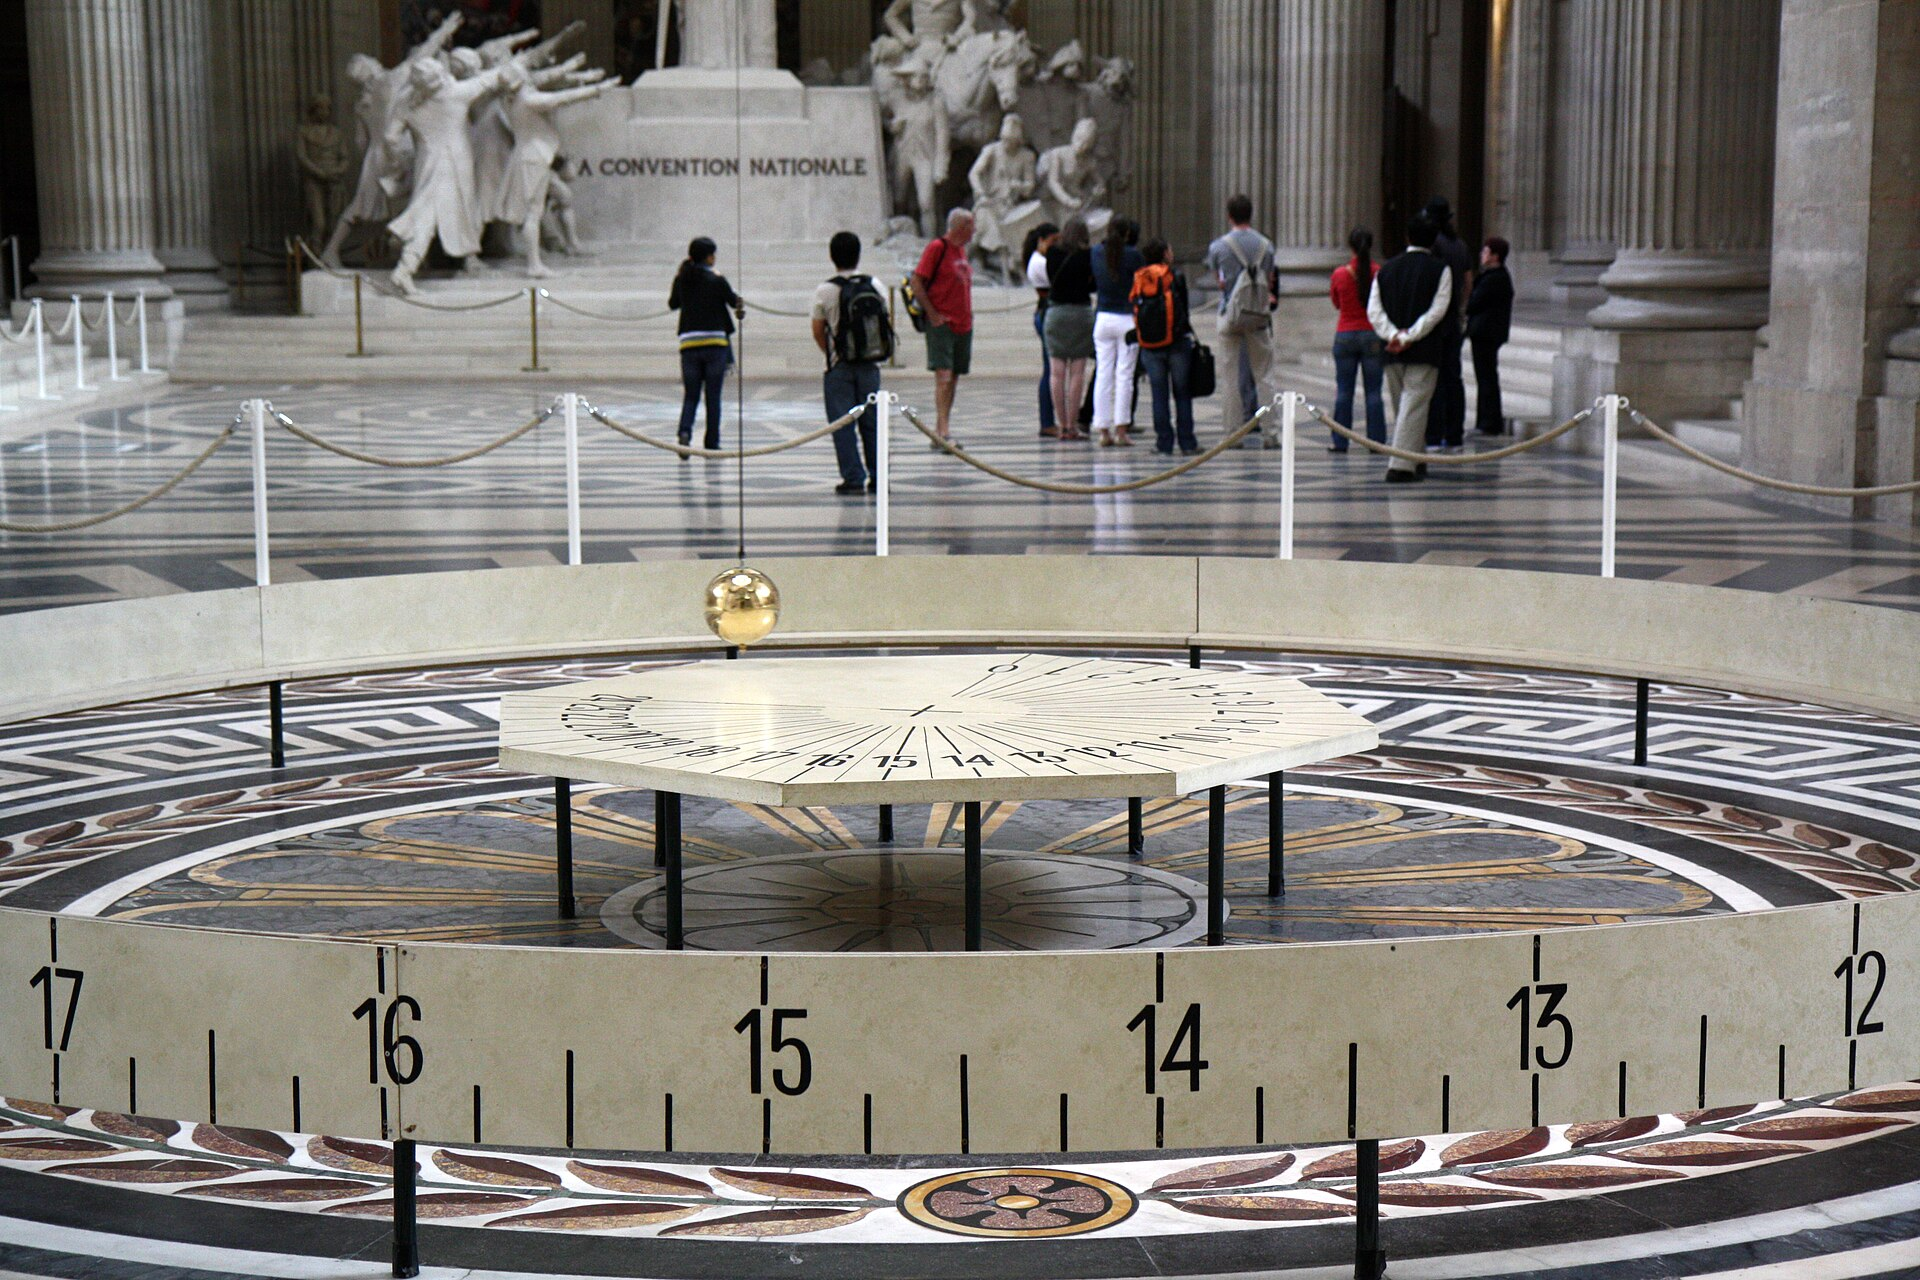
\includegraphics[width=0.6\linewidth]{images/book5/photo-foucault-pantheon.jpg}

{\small بندول فوكو في البانثيون بباريس. \omterm{def:b3:lagrangian-mechanics:coordinates}{إحداثيات معمّمة}، \omterm{def:b3:lagrangian-mechanics:coordinates}{وقيد}، ومرجع يدور ببطء: يظهر دوران القاعة في معادلات الحركة --- وانزياح مستوي التأرجح يتيح لقبو أن يقيس دوران الأرض. الصورة: أولغا خوميتسيفيتش، CC~BY~2.0.}
\end{omfigure}

\section{مسألة: المكنسة التي تقف مقلوبة}

\begin{problem}[{مسألة نهاية الأسبوع --- بندول كابيتزا المقلوب}]\label{pb:b3:lagrangian-mechanics:1}
يستطيع بندول صلب أن يقف مستقرًا \emph{فوق} محوره إذا هُزّ المحور
صعودًا ونزولًا بسرعة كافية --- وهو اكتشاف حلّله كابيتزا سنة 1951،
لافت إلى حدّ يشبه خدعة الحواة، وهو المبدأ الذي تحصر به المجالات
الكهربائية المتذبذبة أيونات مفردة. ونمذج البندول بكتلة نقطية $m$
في طرف قضيب صلب عديم الكتلة طوله $\ell = \qty{40}{cm}$؛ و $\theta$
هي الزاوية عن الشاقول \emph{النازل}؛ و $g = \qty{9.81}{m/s^2}$.

\medskip\noindent\textbf{الجزء الأول --- البندول الصلب.}
المحور مثبَّت في البداية.
\begin{enumerate}
  \item اكتب \omterm{def:b3:lagrangian-mechanics:action}{اللاغرانجية} ومعادلة الحركة.
  \item أعطِ تواتر \omterm{prop:b3:lagrangian-mechanics:modes}{الاهتزازات الصغيرة} $f_0$ حول $\theta =
        0$، وقيمته.
  \item بيّن أن $h = E$ هنا، واستعمل انحفاظها لإيجاد أصغر سرعة
        إطلاق للكرة، في الأسفل، توصلها إلى الأعلى.
  \item خطّط المعادلة بجوار $\theta = \pi$ (بوضع $\theta = \pi +
        \epsilon$) وبيّن أن $\ddot\epsilon = +(g/\ell)\epsilon$: بأيّ
        سرعة ينمو ميل ابتدائي مقداره جزء من ألف من الدرجة؟ أعطِ
        الزمن اللازم لنموّه بعامل $e$.
  \item تسقط مكنسة موازَنة على طرف إصبع في نحو ثانية، ومع ذلك لا
        تقف وحدها أبدًا: اذكر في جملة واحدة ما تقوله المعادلة
        المخطَّطة عن التوازن $\theta = \pi$.
\end{enumerate}

\medskip\noindent\textbf{الجزء الثاني --- هزّ المحور.}
يتذبذب المحور الآن شاقوليًا، وارتفاعه $y_{\text{s}}(t) =
a\cos\Omega t$ مع $a = \qty{2.0}{cm}$ و $\Omega$ قابل للضبط.
\begin{enumerate}[resume]
  \item اكتب إحداثيي الكرة وبيّن أن
        $\vect v^{\,2} = \ell^2\dot\theta^2 -
        2a\Omega\ell\sin(\Omega t)\sin\theta\,\dot\theta +
        a^2\Omega^2\sin^2\Omega t$.
  \item بيّن أن لاغرانجيتين تختلفان بمشتق زمني تام
        $\dd F(q,t)/\dd t$ تعطيان \omterm{thm:b3:lagrangian-mechanics:euler-lagrange}{معادلات أويلر--لاغرانج} نفسها.
  \item باستعمال هذه الحرية، أرجع \omterm{def:b3:lagrangian-mechanics:action}{اللاغرانجية} إلى $L = \tfrac12 m
        \ell^2\dot\theta^2 - ma\Omega^2\ell\cos(\Omega t)\cos\theta +
        mg\ell\cos\theta$. (إرشاد: يجتمع $\sin(\Omega t)\sin\theta\,\dot\theta$
        مع حدّ في $\cos(\Omega t)\cos\theta$ ليعطيا مشتقًا تامًّا؛
        ويجوز إهمال الحدود التي تتعلق بالزمن $t$ وحده.)
  \item استنتج معادلة الحركة
        \[
        \ddot\theta = -\frac{g}{\ell}\sin\theta
         + \frac{a\Omega^2}{\ell}\cos(\Omega t)\sin\theta .
        \]
        وفسّر الحدّ الثاني على أنه استبدال المقدار $g +
        \ddot y_{\text{s}}$ بالثقل: فالبندول يعيش في مصعد.
  \item هل تنحفظ \omterm{prop:b3:lagrangian-mechanics:energy}{دالة الطاقة} $h$ الآن؟ وهل تنحفظ الطاقة؟ وما الذي
        يضخّ الطاقة داخلًا وخارجًا؟
  \item في نظام كابيتزا يكون $a \ll \ell$ و $\Omega \gg \omega_0 =
        \sqrt{g/\ell}$: تحقق من ذلك من أجل $a = \qty{2}{cm}$ و $\ell =
        \qty{40}{cm}$ و $\Omega/2\pi = \qty{40}{Hz}$، وفسّر فيزيائيًّا
        لماذا لا تستطيع الكرة حينئذٍ ملاحقة الإثارة.
\end{enumerate}

\medskip\noindent\textbf{الجزء الثالث --- فصل السريع عن البطيء.}
ابحث عن الحركة في الشكل $\theta(t) = \Theta(t) + \xi(t)$: انزياح
بطيء $\Theta$ يضاف إليه تموّج صغير $\xi$ عند تواتر الإثارة.
\begin{enumerate}[resume]
  \item بإبقاء الحدّ الأكبر وحده في كل طرف، بيّن أن التموّج يحقق
        $\ddot\xi \approx +(a\Omega^2/\ell)\cos(\Omega t)
        \sin\Theta$، مع تجميد $\Theta$ على المقياس الزمني للإثارة.
  \item استنتج $\xi(t) = -(a/\ell)\cos(\Omega t)\sin\Theta$، وتحقق
        من أن سعته صغيرة من رتبة $a/\ell$.
  \item انشر $\sin\theta = \sin(\Theta + \xi)$ حتى المرتبة الأولى في
        $\xi$ وأدخله في معادلة الحركة.
  \item خذ المتوسط على دور إثارة واحد، مع تثبيت $\Theta$:
        باستعمال $\langle\cos\Omega t\rangle = 0$ و
        $\langle\cos^2\Omega t\rangle = \tfrac12$، بيّن أن
        \[
        \ddot\Theta = -\frac{g}{\ell}\sin\Theta
         - \frac{a^2\Omega^2}{2\ell^2}\sin\Theta\cos\Theta .
        \]
  \item بيّن أن هذه حركة في الكمون الفعّال
        \[
        U_{\text{فعّال}}(\Theta) = mg\ell\Big({-\cos\Theta}
         + \frac{a^2\Omega^2}{4g\ell}\sin^2\Theta\Big) .
        \]
  \item قارن بالخرزة على الحلقة الدوّارة
        (\cref{ex:b3:lagrangian-mechanics:hoop}): الرياضيات نفسها،
        وإشارة الحدّ الجديد معاكسة --- فما الذي يفعله الهزّ بتوازن
        \emph{الأسفل} ولم يفعله الدوران؟
  \item ارسم $U_{\text{فعّال}}$ تقريبيًا من أجل إثارة بطيئة وأخرى
        سريعة، وصف كل توازن واستقراره في كل حالة.
\end{enumerate}

\medskip\noindent\textbf{الجزء الرابع --- المكنسة تقف.}
\begin{enumerate}[resume]
  \item بنشر $U_{\text{فعّال}}$ بجوار $\Theta = \pi$، بيّن أن الوضع
        المقلوب مستقر بالضبط عندما يكون
        \[
        a^2\Omega^2 > 2g\ell .
        \]
  \item احسب تواتر الإثارة الحرج $f_{\text{c}} =
        \Omega_{\text{c}}/2\pi$ لبندولنا، وكذلك السرعة القصوى
        للمحور $a\Omega_{\text{c}}$ والتسارع الأقصى
        $a\Omega_{\text{c}}^2$ (بواحدة $g$) الذي يتطلبه.
  \item عند $\Omega = 2\Omega_{\text{c}}$، أوجد تواتر التمايل
        البطيء للبندول الواقف حول $\Theta = \pi$، وقيمته؛ وتحقق
        من أنه بطيء فعلًا بالمقارنة مع الإثارة.
  \item ومع بقاء $\Omega = 2\Omega_{\text{c}}$، ما سعة التموّج
        $\xi$ عند $\Theta$ تبتعد قليلًا عن $\pi$، بالدرجات، من
        أجل $a/\ell = 0.05$؟ وهل تفضح صورة فوتوغرافية الخدعة؟
  \item إلى أيّ حدّ يمكن أن تميل المكنسة عن الشاقول وتعود؟
        بيّن أن بئر الوقوف تمتد على $|\Theta - \pi| <
        \arccos(2g\ell/a^2\Omega^2)$، وقدّرها عند $\Omega =
        2\Omega_{\text{c}}$.
  \item يُبقي البهلوان مكنسة موازَنة على طرف إصبع ساكن قائمة
        أيضًا --- فبأيّ آلية مختلفة تمامًا؟ سمِّ الخاصية التي
        يتميز بها بندول كابيتزا ولا تحتاج إلى تغذية راجعة.
  \item لخّص النتيجة الموسومة: محور يُهزّ بسعة
        \qty{2}{cm} عند \qty{45}{Hz} --- أي ضعف التواتر الحرج ---
        يمسك بندولًا طوله \qty{40}{cm} مقلوبًا، في بئر تمتد إلى
        نحو $75^\circ$ عن الشاقول، ويتمايل برفق عند
        \qty{1.4}{Hz} تقريبًا. فأين في الفيزياء يُستعمل هذا
        الحصر بالتوسيط نفسه لإمساك جسيم مشحون مفرد؟
\end{enumerate}
\end{problem}
